%! Author = Saeid Yazdani
%! Date = 9/6/2024


\section{Compensation Network Results}
\label{sec:isolated-preamp-meas}

The compensation network can be used to tune the bandwidth of pre and power
amplifiers to a specific value.
Tuning the bandwidth can help reduce noise by filtering out high-frequency
interference, resulting in a cleaner signal and a better signal-to-noise ratio.
Stability will also be improved by minimizing the risk of oscillations.

Using the provisioned jumpers and test points,
pre-amplifier was tested in isolation for \emph{current consumption} and
\emph{bandwidth} under various combinations of compensation values.
The equivalent circuit for this test is shown in
\autoref{fig:test-preamp-isolation-circuit}.

\subsection*{Test Conditions:}

\begin{itemize}[topsep=8pt,itemsep=4pt,partopsep=4pt, parsep=4pt]
    \item All low voltage supplies active
    (\SI{\pm15}{\volt}, \SI{\pm5}{\volt}, \SI{\pm3.3}{\volt})
    \item Tracking supply set to \SI{\pm50}{\volt}
    \item Fixed feedback series RC values of  \SI{4.7}{\kilo\ohm} and
    \SI{4.7}{\nano\farad} on the amplifier
    \item Using only one resistance value for the compensation network
    (PRECMP\_R[1] in series with PRECMP\_R[2] = \SI{15.1}{\ohm}) but switching
    between
    all capacitances individually (\SI{100}{\pico\farad} to \SI{22}{\nano\farad})
    according to \autoref{sec:compensation-network-values}.
\end{itemize}

\begin{figure}[h]
    \centering
    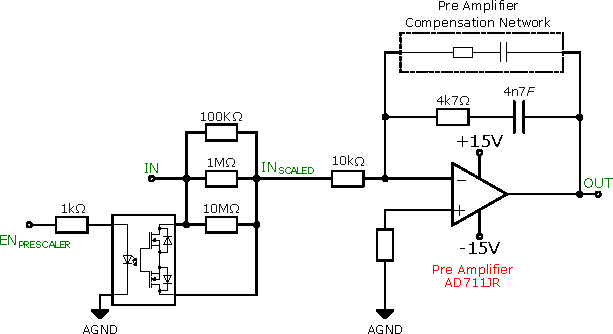
\includegraphics[width=0.85\textwidth]
    {figures/tests/preamp-test-circuit}
    \caption[Pre-Amplifier Isolation Test Circuit]{
        The equivalent circuit for testing the pre-amplifier in isolation.
    }
    \label{fig:test-preamp-isolation-circuit}
\end{figure}



The bandwidth measurements were carried out with an input voltage swing of
\SI{\pm10}{\volt}, once without prescaler\footnote{There is a relay-controlled divider network right before the input
stage that can divide the input signal by 10.} disabled and once with prescaler
set to $10:1$.

\subsection*{Measurement Results:}
With 8 resistors and 8 capacitors, a large combination of values is possible,
allowing us to fine-tune the bandwidth as required, therefore the results
presented here are for only a combination of one resistance value and 8
capacitance value.
The result is presented in \autoref{tab:combined_capacitor_bandwidth}.

\begin{table}[h!]
    \centering
    \resizebox{\linewidth}{!}{%
    \begin{tabular}{lcc}
        \toprule

        \small\textbf{Capacitor} & \small\textbf{B/W 3dB (Prescaler Disabled)} & \small\textbf{B/W 3dB (Prescaler 10:1)} \\
        \midrule
%        \SI{0}{\pico\farad}      & \SI{4200}{\kilo\hertz}                      & --                                      \\
        \SI{100}{\pico\farad}    & \SI{300}{\kilo\hertz}                       & \SI{225}{\kilo\hertz}                   \\
        \SI{220}{\pico\farad}    & \SI{120}{\kilo\hertz}                       & \SI{100}{\kilo\hertz}                   \\
        \SI{470}{\pico\farad}    & \SI{60}{\kilo\hertz}                        & \SI{50}{\kilo\hertz}                    \\
        \SI{1}{\nano\farad}      & \SI{30}{\kilo\hertz}                        & \SI{23}{\kilo\hertz}                    \\
        \SI{2.2}{\nano\farad}    & \SI{12}{\kilo\hertz}                        & \SI{9}{\kilo\hertz}                     \\
        \SI{4.7}{\nano\farad}    & \SI{6}{\kilo\hertz}                         & \SI{5}{\kilo\hertz}                     \\
        \SI{10}{\nano\farad}     & \SI{2.5}{\kilo\hertz}                       & \SI{2.4}{\kilo\hertz}                   \\
        \SI{22}{\nano\farad}     & \SI{1.2}{\kilo\hertz}                       & \SI{1.2}{\kilo\hertz}                   \\
        \bottomrule
    \end{tabular}
    }
    \caption[PreAmplifier Compensation Network Measurement]{
        Comparison of effect of changing capacitor values inthe compensation network of the pre amplifier.
    }
    \label{tab:combined_capacitor_bandwidth}
\end{table}

The difference in frequency between the results can be attributed to
signal amplitude and the capacitance of the analog relay used in the switching
of the prescaler divider network path.
It was observed that disabling the compensation will cause an
output resonance at \SI{5}{\mega\hertz} and the current draw of the amplifier
is \SI{13}{\milli\ampere} on average.
